\documentclass[11pt,a4paper]{article}
\usepackage[margin=22mm]{geometry}
\usepackage{fontspec,babel}
\babelprovide[main,import]{russian}
\babelfont{rm}{Times New Roman}
\babelfont{sf}{Arial}
\usepackage{amsmath,booktabs,graphicx,xcolor,caption,hyperref}
\hypersetup{colorlinks,allcolors=blue!45!black,
  pdftitle={Прямая проверка скоростной поправки в идеальной 12-электродной ловушке}}
\captionsetup{font=small,labelfont=bf,hypcap=false}
\graphicspath{{outputs/effective_reconstruction/p4_transfer/v1/report/}{./}}
\setlength{\parindent}{0pt}
\setlength{\parskip}{4pt}
\setlength{\emergencystretch}{2em}
\begin{document}
{\sffamily\small ПРИЛОЖЕНИЕ К ОТЧЁТУ ОБ ЭФФЕКТИВНОЙ ДИНАМИКЕ \hfill P4 / v1}\par
\vspace{0.45cm}
{\sffamily\LARGE\bfseries Прямая проверка скоростной поправки\\
в 12-электродной ловушке\par}
\vspace{0.2cm}
{\small 8 ноября 2026 г. \quad $q=10^{-12}$ Кл, $m=10^{-15}$ кг, $U_0=250$ В, $f=100$ кГц}

\medskip
Модель E предсказывает наблюдаемую прецессию на новых стартах при 0,75 и
1,25 мм. Перестановка фаз ABC $\to$ ACB меняет знак поворота при одном и том
же стартовом азимуте. В модели E энергия удержания $B_6r^6$ дополнена
скоростным ускорением
\[
\gamma(r)J\dot{\mathbf R},
\qquad
\gamma(r)=\sigma\,(1{,}26760747\,\text{с}^{-1})
\left(\frac{r}{1\,\text{мм}}\right)^4,
\qquad (\sigma_{\rm ABC},\sigma_{\rm ACB})=(+1,-1).
\]
Здесь $J(x,y)=(-y,x)$, $B_6=22{,}12392402$ Дж\,м$^{-6}$.
Коэффициенты взяты из исходной калибровки поля. Сравнение проведено
на общем физическом времени с центрированным RF-средним прямой динамики A
на сетке P4 h35. Скорость поворота определена по углам радиальных разворотов.

\begin{center}
\small
\begin{tabular}{@{}lrrrrrr@{}}
\toprule
Старт, мм & \multicolumn{2}{c}{Поворот, $^\circ$/с}
  & \multicolumn{2}{c}{RMS, \%} & \multicolumn{2}{c}{Максимум, \%} \\
\cmidrule(lr){2-3}\cmidrule(lr){4-5}\cmidrule(l){6-7}
 & A & E & B & E & B & E \\
\midrule
0,75 ABC & $+3{,}53248$ & $+3{,}53331$ & 0,23415 & 0,000125 & 0,56946 & 0,000214 \\
0,75 ACB & $-3{,}53694$ & $-3{,}53331$ & 0,23444 & 0,000258 & 0,57018 & 0,000587 \\
1,25 ABC & $+27{,}24813$ & $+27{,}26324$ & 1,08373 & 0,001623 & 2,63550 & 0,002847 \\
1,25 ACB & $-27{,}32063$ & $-27{,}26324$ & 1,08663 & 0,002538 & 2,64251 & 0,005573 \\
\bottomrule
\end{tabular}
\end{center}

\begin{center}
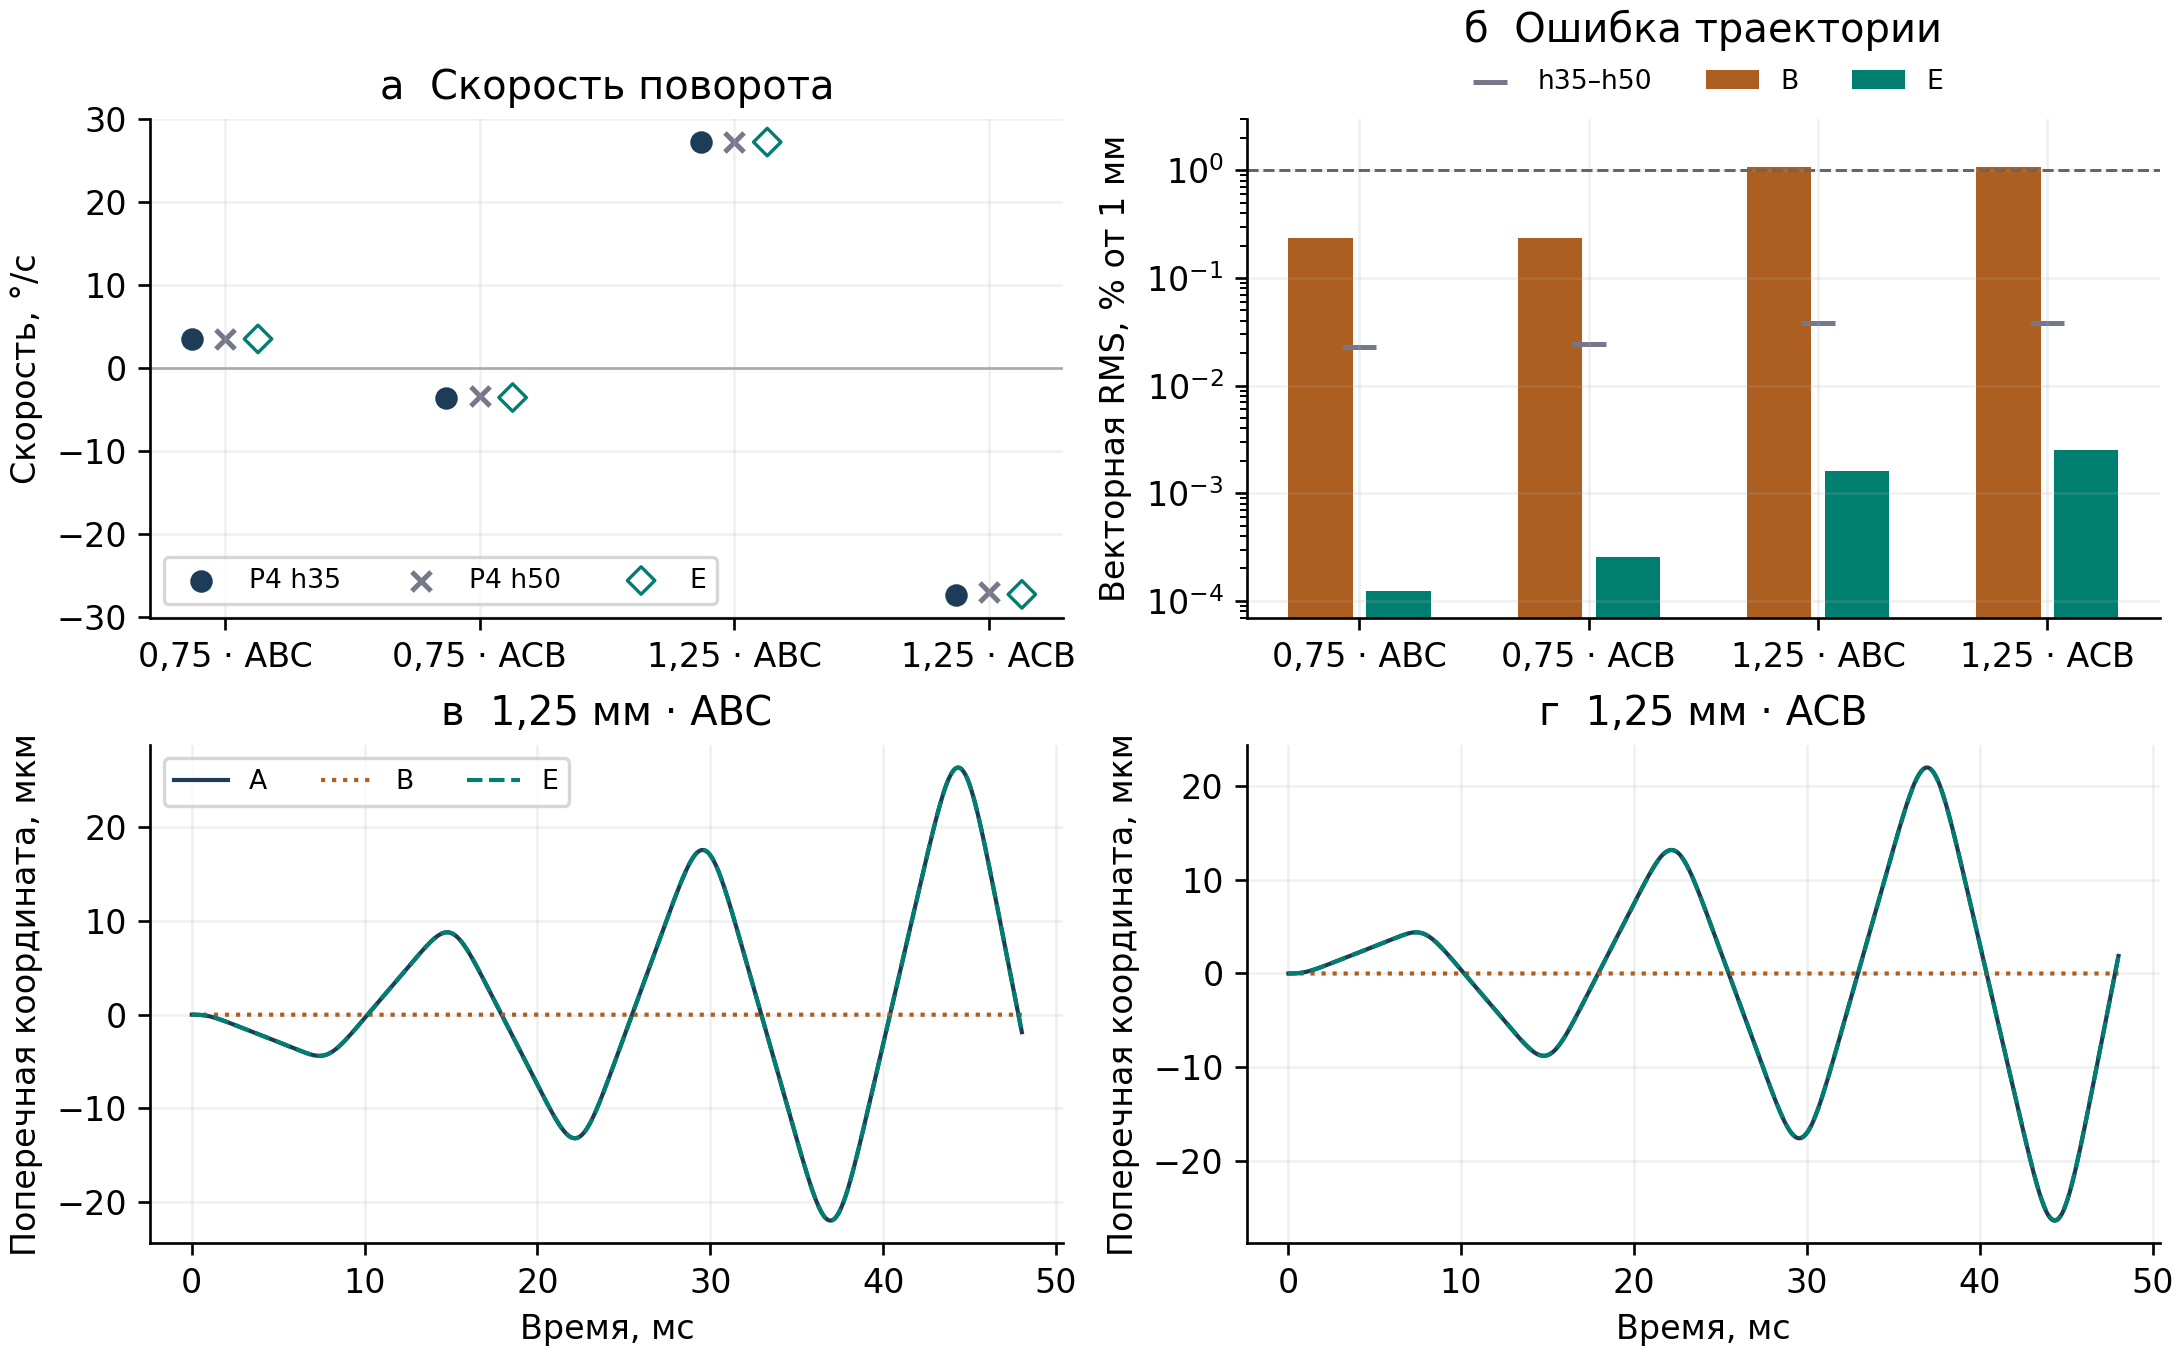
\includegraphics[width=\linewidth]{p4_transfer.png}
\captionof{figure}{Скорость поворота, векторная ошибка в процентах от 1 мм и
поперечные траектории при 1,25 мм. В панели б штрихи показывают RMS между
сетками, а пунктир отмечает физический порог 1\%. В панелях в и г A и E
почти совпадают на масштабе графика.}
\end{center}

\newpage
\section*{Численные контроли и интерпретация}

Два радиуса и две последовательности фаз рассчитаны на сетках P4 h35 и h50
с максимальными шагами DOP853 $T_{\rm RF}/50$ и $T_{\rm RF}/100$.
В каждом из 16 расчётов пройдено около 3,25 медленного периода.
Стартовые азимуты составили 0,23 и 0,31 рад, начальные RF-фазы 0,70 и
1,10 рад соответственно. Для одного старта все сетки и шаги использовали
побитно одинаковое полное начальное состояние.

\begin{center}
\small
\begin{tabular}{@{}lrr@{}}
\toprule
Контроль & Векторная RMS, \% & Изменение скорости, $^\circ$/с \\
\midrule
Сетки h35/h50 при $T_{\rm RF}/100$ & 0,02279--0,03790 & 0,03369--0,30996 \\
Шаг $T_{\rm RF}/50$ и $T_{\rm RF}/100$ & $\leq 7{,}18\times10^{-9}$ & $\leq 8{,}85\times10^{-8}$ \\
Обратная карта и RF-среднее h35 & --- & $\leq 6{,}0\times10^{-8}$ \\
Сырой строб и RF-среднее h35 & --- & $\leq 0{,}0545$ \\
\bottomrule
\end{tabular}
\end{center}

Все четыре старта удовлетворяют заранее заданным критериям E.
Улучшение относительно B по векторной RMS и скорости поворота превышает
удвоенный наблюдаемый численный разброс. Ошибки E приведены относительно
h35. Межсеточные различия задают отдельный масштаб чувствительности.
Сверены хеши итоговых файлов 16 запусков, 104 контрольных точек
и журналов переходов.

При 1,25 мм B превышает порог 1\% RMS при ошибке периода около 0,00023\%.
Нечётные по направлению вращения скорости равны $+3{,}53471$ и
$+27{,}28438^\circ$/с. Их отношение 7,719 близко к
$(1{,}25/0{,}75)^4=7{,}716$. Поскольку с радиусом меняются также азимут и
RF-фаза, это проверка двух прогнозов. Для независимой оценки показателя по
радиусу нужна серия при фиксированных азимуте и фазе. Малая чётная
компонента на h35 лежит ниже наблюдаемого межсеточного разброса.

\section*{Независимый частотный контроль}
В чистом вращающемся октуполе измерена разность поперечных ускорений
на радиусе 1 мм для противоположных радиальных скоростей при фиксированном
напряжении. Средние оценки $\gamma(1\,\text{мм})$ составили 2,475314,
1,267605 и 0,461957 с$^{-1}$ при 80, 100 и 140 кГц. Показатель аппроксимации
равен $-2{,}99967$ при предсказании $-3$. Максимальное относительное
отклонение отдельной оценки от прогноза составило 0,0418\%.

\section*{Область применимости}
Радиальный псевдопотенциал воспроизводит период и радиальную амплитуду,
а ведущая скоростная поправка воспроизводит поворот линии колебаний.
На новых радиусах результат проверен на 3,25 медленного периода, в исходном
исследовании при 1 мм --- до 10,25 периода. Для 50 периодов нужна отдельная
глобальная проверка сходимости по сетке и шагу.
Протокол, прогнозы и численные таблицы хранятся в репозитории.

\end{document}
